\section{Experiments}


\subsection{Datasets}

The six used datasets are summaries in Table.~\ref{tbl:dataset}.
\emph{DIGITS} is a subset of the optical recognition of handwritten digits dataset~\cite{kaynak1995methods} of 8x8 grayscale images.
\emph{COIL20} \cite{nene1996} is a dataset of 32x32 grayscale pictures of 20 rotated objects.
\emph{FASHION\_1K} contains 1000 grayscale images of size 28x28, sampled from Fashion-MNIST\cite{xiao2017/online} clothing dataset.
The grayscale images from there above datasets are normalized and used directly in the DR methods.

\emph{FASHION\_MOBILENET} contains features extracted from a subset of Fashion Product images dataset~\cite{fashionproduct}.
The MobileNet\cite{} with pre-trained weights from ImageNet is used for feature extraction, a transfer learning technique that uses the representation of the learned network (trained on a large-scale image classification task) to extract meaningful features for new samples.
The last fully connected layer of the network is replaced by a global average pooling layer\cite{} to obtain the flatten output vector of 1280 dimensions.
To speed up the DR methods, PCA is then applied to take only 75 features.

\emph{5NEWS} contains the text of 5 groups selected from the 20 Newsgroups dataset which are converted to a matrix of token counts via TF-IDF method.
The count vectors are then fed into Latent Dirichlet Allocation (LDA) model to extract 15 hidden topics, which are 15 features used for DR methods.

The open \emph{NEURON\_1K}~\cite{neuron1k} dataset contains 1301 Brain Cells from an E18 Mouse, processed and provided by 10X Genomics, a company who provides chromium single cell gene expression solution and publics several genetic datasets.\footnote{https://www.10xgenomics.com/resources/datasets/, The datasets are licensed under the Creative Commons Attribution license.}
The processed data have 10 PCA features and labeled in 6 classes found by a graph-based clustering method.


\begin{table*}[width=\textwidth,cols=6,pos=h]
\caption{Description of six selected datasets with samples for the image datasets.}\label{tbl:dataset}
\begin{tabular}{m{3cm} m{4.8cm} m{8cm}}
\toprule
Dataset name & Samples & Description \\
\midrule

\emph{COIL20}
    & 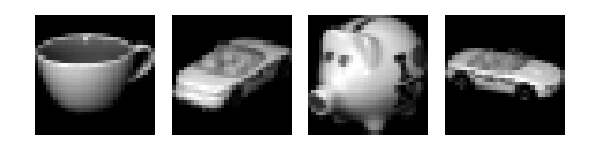
\includegraphics[width=\linewidth]{COIL20_samples}
    & 1440 grayscale images of size 32x32, belonging to 20 classes.
    The raw images of 1024 dimensions are used directly for the DR methods.\\

\emph{DIGITS}
    & 
\includegraphics[width=\linewidth]{DIGITS_samples}
    & 1797 grayscale images of size 8x8 of 10 digits.
    The raw images of 64 dimensions are used directly for the DR methods.\\

\emph{FASHION\_1K}
    & 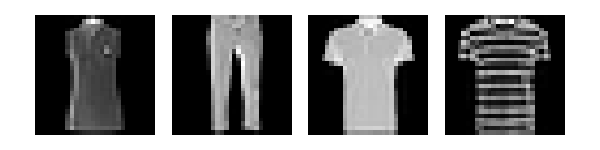
\includegraphics[width=\linewidth]{FASHION1000_samples}
    & 1000 grayscale images of size 28x28 of 10 classes, sampled from Fashion-MNIST dataset.
    The raw images of 768 dimensions are used directly for the DR methods.\\

\emph{FASHION\_MOBILENET}
    & 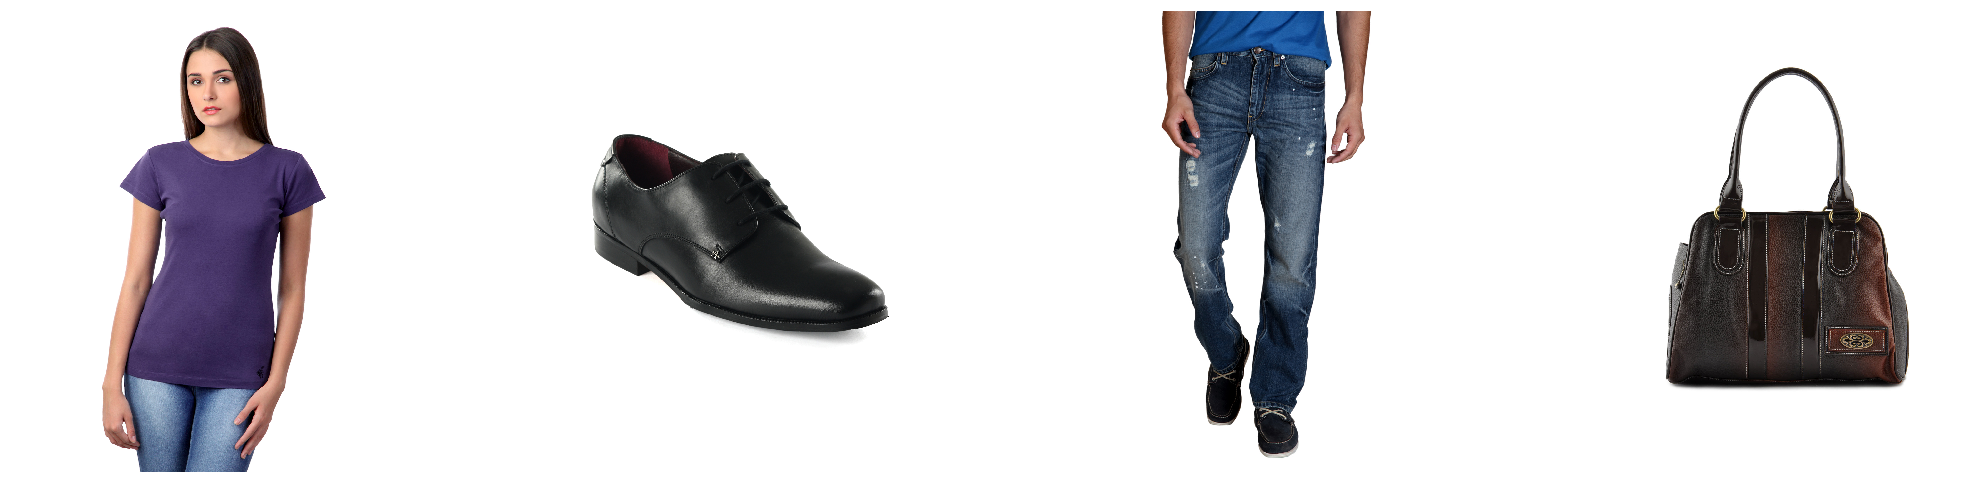
\includegraphics[width=\linewidth]{FASHION_PRODUCT_samples}
    & 1494 color images of various sizes belonging to 7 classes
    (\path{'Bags', 'Bottomwear', 'Jewellery', 'Sandal', 'Shoes', 'Topwear', 'Watches'}),
    sampled from Fashion Product images dataset.\\

\emph{5NEWS}
    & 
\includegraphics[width=\linewidth]{20NEWS5_samples}
    & 5 groups of 2957 emails selected from 20Newsgroups dataset,
    including \path{'rec.autos', 'rec.sport.baseball','sci.crypt', 'sci.space', 'comp.sys.mac.hardware'}. \\

\emph{NEURON\_1K}
    &
    & 1301 brain cells from a combined cortex, hippocampus and subventricular zone of an E18 mouse. \\

\bottomrule
\end{tabular}
\end{table*}


\subsection{Constraint Generation}

The input for our proposed constraint preserving scores is ensemble of constraints in form of similar links and dissimilar links.


\subsection{Proof of Concept}


For the flexibility:
We design the score independently to the DR methods.
As shown in the above experiments, the constraint score can be used to evaluate the embedding quality of t-SNE or UMAP.
These well-known methods are widely used since they have ability to preserve the neighborhood information, i.e. to make the data points in the same class close together.
In this way, the local structure of the data is highlighted.
But as pointed out in the distill article ``How to use t-sne effectively'' by \citet{wattenberg2016use}, the distance between clusters might not mean anything.

The hyperparameters of t-SNE and UMAP make these methods difficult to use correctly but also make them flexible.
These methods can produce different visualizations and reveal different hidden structures in the data.
To evaluate the embedding quality of such flexible methods, we need a flexible score.
The state of the art $AUC_{log}RNX$ metric or the BIC-based score has no flexibility to capture different visualization results.

$AUC_{log}RNX$ metric evaluates how the neighborhood information is preserved.
The BIC-based score evaluates the trade-off between KL loss and the value of perplexity in t-SNE.
In contrast, the $f_{score}$ evaluates how the constraints are preserved.

$f_{score}$ takes a set of constraints as input to find the best visualization which respects the constraints.
Naturally, the constraints generated from the class labels reflect the class-relationship between the data points in the same class.